\documentclass{standalone}
\usepackage{ tikz }
\usepackage{ amssymb }
\usepackage{ xparse }
\input{macros/all}

\begin{document}
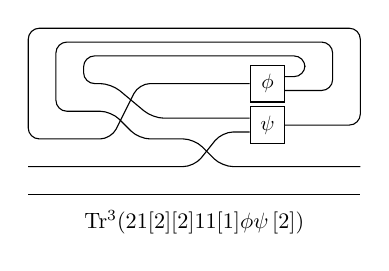
\begin{tikzpicture}[yscale=-1,x=1em,y=1em]

    \draw [rounded corners] (8,1.25) -- (4.5,1.25) -- (3,0) -- (2,0) -- (2, -1) -- (10, -1) -- (10, -0.25) -- (9.25,-0.25);
    \draw [rounded corners] (8,1.75) -- (7,1.75) -- (6,3) -- (0,3);
    \draw [rounded corners] (8,0) -- (4,0) -- (3,2) -- (0,2) -- (0,-2) -- (12,-2) -- (12,1.5) -- (9.25,1.5);
    \draw [rounded corners] (12,3) -- (7,3) -- (6,2) -- (4,2) -- (3,1) -- (1,1) -- (1,-1.5) -- (11, -1.5) -- (11, 0.25) -- (9.25, 0.25);
    \draw [] (0,4) -- (12,4);

    \node [draw, minimum height = 1.25em, minimum width = 1.25em, anchor=west] at (8,0) {\scalebox{0.75}{$\phi$}};
    \node [draw, minimum height = 1.25em, minimum width = 1.25em, anchor=west] at (8,1.5) {\scalebox{0.75}{$\psi$}};

    \node [anchor=center] at (6,5) {\scalebox{0.8}{Tr$^3(\swap{2}{1} \tensor \id[2] \seq \id[2] \tensor \swap{1}{1} \tensor \id[1] \seq \phi \tensor \psi \tensor \,\id[2])$}};

\end{tikzpicture}
\end{document}
